\section{Project Overview}

    Physical infrastructure is a large and complicated subject, encompassing everything from running water to mains electricity. Below I have listed the main features included in physical infrastructure:

    \begin{itemize}
        \item \textbf{Transportation:} Road and highway networks; Mass transit systems; Railways; Canals; Seaports; Airports; Bicycle paths / pedestrian walkways

        \item \textbf{Energy:} Electrical power network; Natural gas pipelines; Petroleum pipelines; Coal production and processing

        \item \textbf{Water management:} Drinking water supply; Sewage collection; Drainage systems; Irrigation systems; Flood control systems; Coastal management

        \item \textbf{Communications:} Postal service; Telephone networks; Mobile phone networks; Television and radio stations; Internet services; Communications satellites; Undersea cables

        \item \textbf{Solid waste management:} Landfills; Incinerators; Hazardous waste disposal
    \end{itemize}

    Computer modelling systems could be developed for any one of these areas, allowing users to prototype infrastructure designs before the costly process of constructing it. For this project I have chosen to focus on the Transportation sector, as it can include some of the most expensive forms of infrastructure.

    Naturally the major responsibility of transportation infrastructure goes towards the construction and maintenance of road networks, including but not limited to junctions, roundabouts, highways and traffic lights.
    These networks can get very complicated and difficult to manage, for example the UK's so called "spaghetti junction" in Birmingham.

    \begin{figure}[h]
        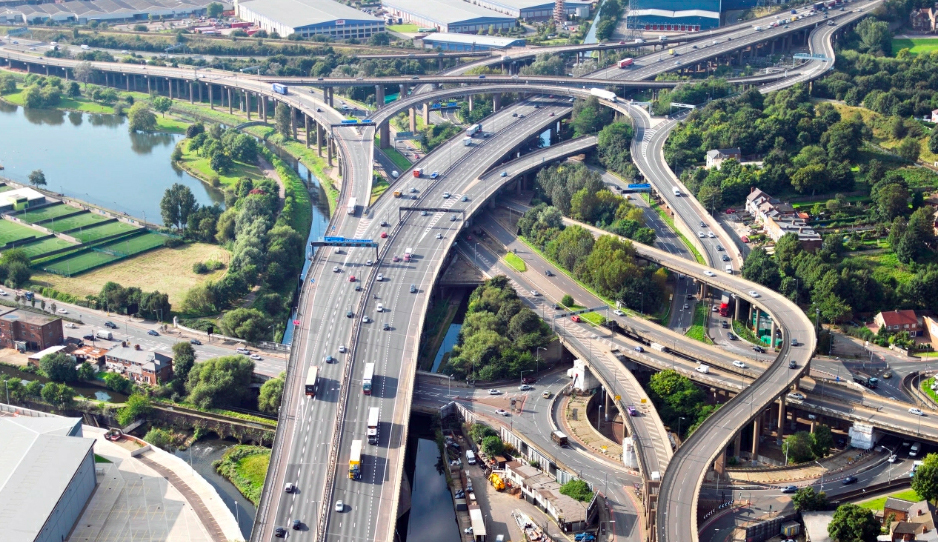
\includegraphics[width=0.5\textwidth]{Spaghetti-Junction.jpg}
        \centering
        \caption{Birmingham's "Spaghetti junction" \cite{Spaghetti-Junction}}
    \end{figure}

\section{The Problem}

    Development of transportation is a very expensive and time consuming process, so being able to evaluate the efficiency and cost-effectiveness of road layouts beforehand would be very beneficial. This project aims to develop a road network simulator that can be used to evaluate the efficiency of inputted designs under a range of different traffic conditions.

    \subsection{End user}

\section{Current Systems}

    \subsection{AnyLogic - Road Traffic Simulation Software}

        AnyLogic - Road Traffic Simulation Software \cite{AnyLogic} is an industry-level program used for analysing traffic patterns and behaviours, below are a couple images of the program.

        \begin{figure}[ht]
            \centering
            \begin{minipage}{0.3\textwidth}
                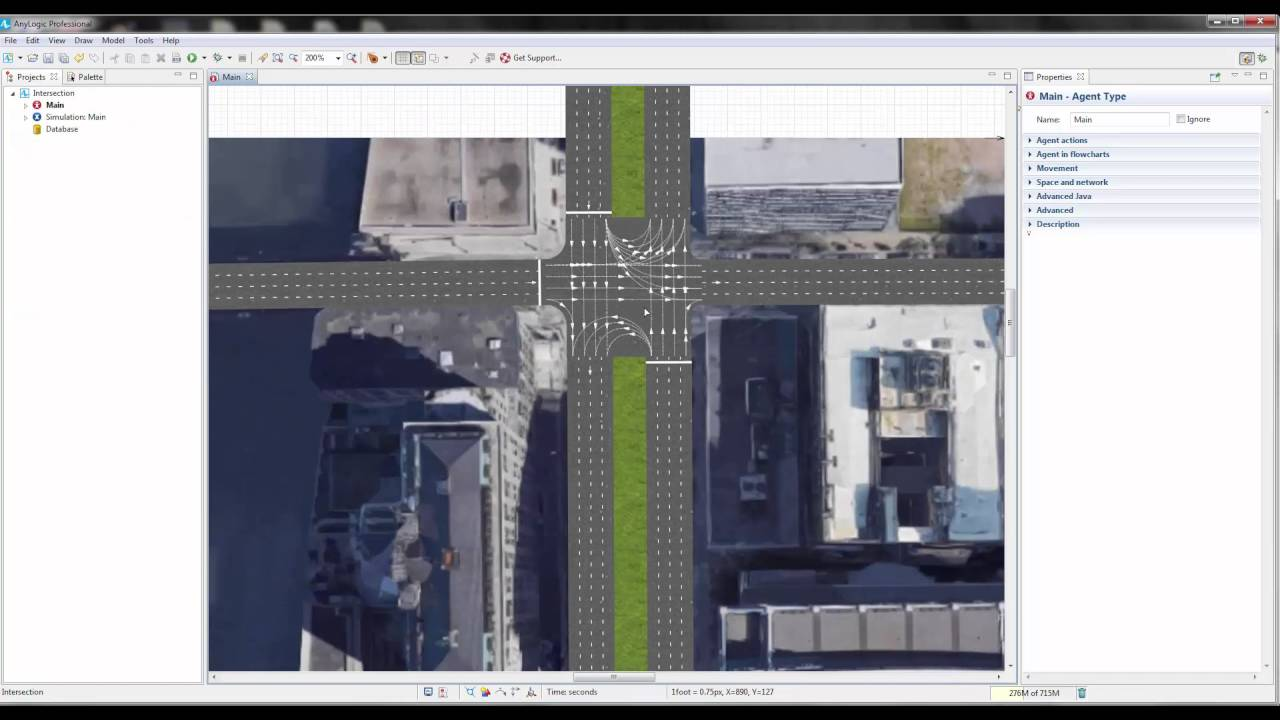
\includegraphics[width=0.8\textwidth]{anylogic-image-1.jpg}
                \caption{Happy Smiley}
            \end{minipage}
            \begin{minipage}{0.3\textwidth}
                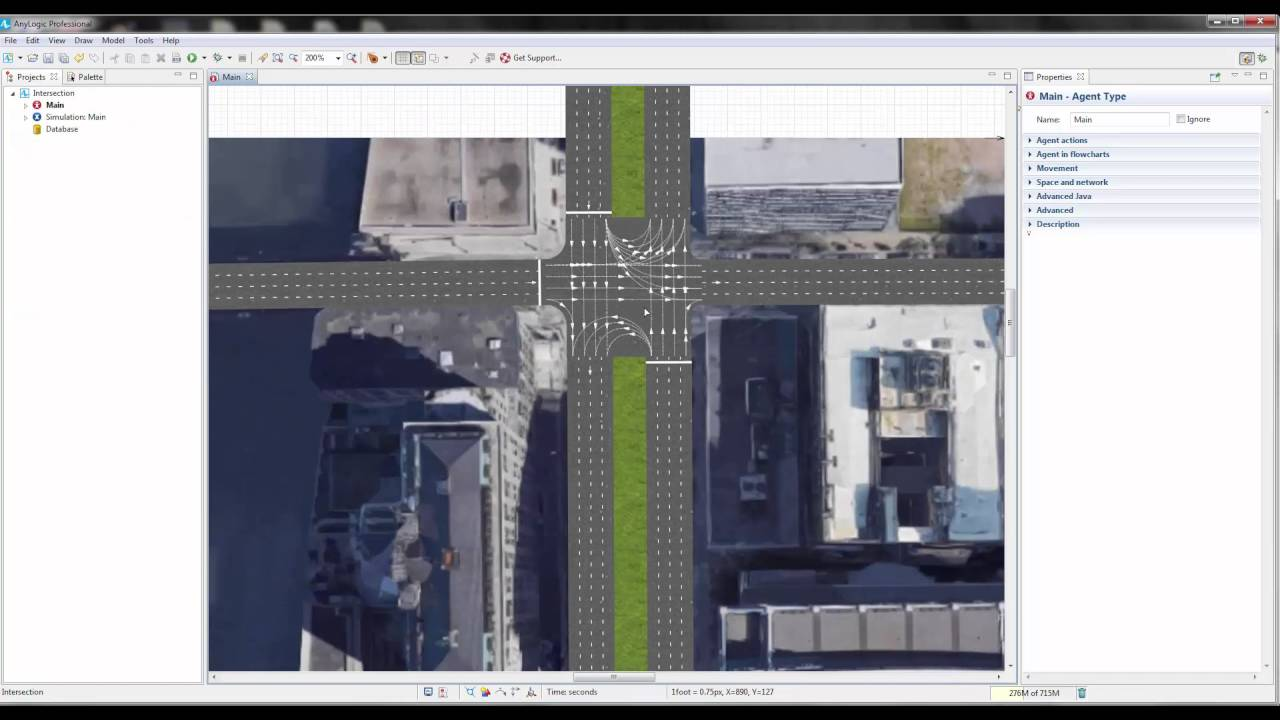
\includegraphics[width=0.8\textwidth]{anylogic-image-1.jpg}
                \caption{Sad Smiley}
            \end{minipage}
            \begin{minipage}{0.3\textwidth}
                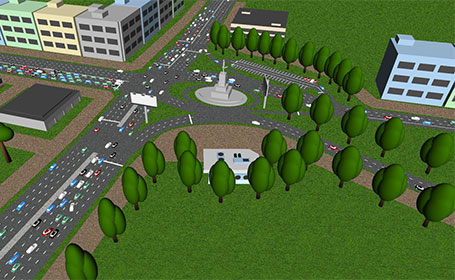
\includegraphics[width=0.8\textwidth]{anylogic-image-3.jpg}
                \caption{Sad Smiley}
            \end{minipage}
        \end{figure}

    \subsection{SOUND}

    \subsection{Eclipse SUMO}

\section{Research}

\section{Proposed Solution}

\section{Objectives}
